\documentclass[./tfe]{subfiles}

\begin{document}

Un patient de 77 ans s’est présenté en février 2019 au service des urgences de l'hôpital Brugmann pour des douleurs thoraciques dorsales persistantes évoluant depuis une semaine, non soulagées par des analgésiques. Apparition récente de dysphagie aux solides et liquides, ainsi que de l’hémoptysie. Le patient est sous Clindamycine depuis 3 jours pour une suspicion d’infection urinaire.

Son histoire médicale révèle une hypertension artérielle, une cryoablation de la voie lente d’une tachycardie de rentrée en 2012, un diabète, un anévrisme aortique thoracique descendant stable, un pontage prothétique fémoral-poplitée pour thrombose d'artère fémorale gauche en 2012 sous sintrom. Arrêt de tabac depuis deux ans, pas de consommation d’alcool et pas d’allergies connues.

À l'examen physique : FC : 112 bpm ; PA : 112/48 mmHg ; T: \SI{35.2}{\celsius}; Saturation en O2: 98\%; FR: 20irpm; glycémie: 209; Glasgow 15, cachexie, pâleur, eupnéique au repos. Jugulaires non turgescentes, absence de souffle carotidien, à l’auscultation cardiaque B1 et B2 réguliers, souffle systolique présent sur foyer mitral 4/6 irradié vers l'aisselle gauche. À l’auscultation pulmonaire murmure vésiculaire diminué sur poumon gauche, râles crépitants sur la base gauche. Abdomen sans particularité à part une sensibilité à la palpation.

\begin{figure}[!h]
    \centering
    
    \begin{subfigure}[b]{.5\textwidth}
        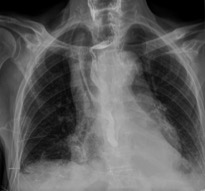
\includegraphics[width=.9\textwidth]{images/rx_esophage_devie_a_droite.jpg}
        \caption{flèche: œsophage dévié à droite}
        \label{fig:rx_1}
    \end{subfigure}%
%
    \begin{subfigure}[b]{.5\textwidth}
        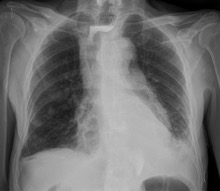
\includegraphics[width=.9\textwidth]{images/rx_epanchement_pleural_bilateral.jpg}
        \caption{* indique l’épanchement pleural bilatéral}
        \label{fig:rx_2}
    \end{subfigure}
    
\caption{Radiographie de thorax de face}
\label{fig:rx_esophage}
\end{figure}

À la biologie, Hb 11.2 g/dL (N= 13-18 g/dL); Gb 14,57 x 103/\si{\micro\liter} (N= 3,5 – 11 x 103/\si{\micro\liter} ); neutrophiles: 79,1\% (N = 40 – 75\%) ; CRP: 200 mg/L (N < 5 mg/L); INR> 9 U (N = 0,95 – 1,31 U); DFG: 26 mL/min/1,73 \si{\cubic\meter} ; lactate: 2,9 mmol/L (0,7 – 2,0 mmol/L); glycémie: 234 mg/dL (70-100 mg/dL).

La radiographie du thorax a montré une déviation œsophagienne droite avec un épanchement pleural bilatéral. (Fig 1 )

Au CT Scan du thorax ( Fig 2) , visualisation de rupture d'un anévrisme aortique descendant avec saignement actif antérieur, présence d'un gros hématome comprimant l'œsophage, mesurant 67X64 mm, sténose de l'artère rénale gauche avec atrophie rénale gauche (connue depuis 2012). Aorte abdominale sans modifications. Épanchement pleural bilatéral. Hernie hiatale volumineuse. Le patient a été traité avec du Konakion et Cofact pour l’INR à 9, du Tradonal afin de soulager la douleur. Il a aussi été transfusé de quatre concentrées d’hématies à cause de la chute de l’hémoglobine (de 11,2 à 8,4 g/dL). Le patient a été admis à l'USI avec une hypotension de 95/65 mmHg. Le lendemain, deuxième jour d'hospitalisation (J2), le patient a bénéficié d'un traitement de dissection aortique type Stanford B compliquée par la pose de deux endoprothèses (Valiant TM Medtronic) de 150 mm de long, la première placée à 5 cm après l'émergence de l'artère sous-clavière gauche et la deuxième avant le tronc cœliaque (Fig3- aucune image qui montre l’endoprothèse entière). Le syndrome inflammatoire initial du patient a continué d’augmenter avec la CRP passant de 200.1 mg/L à 348 mg/L. Au J4, le patient a bénéficié d’un placement de drain thoracique à droite avec une amélioration progressive et importante des paramètres biologiques.

\begin{figure}[!h]
    \centering
    \begin{subfigure}[b]{.5\textwidth}
        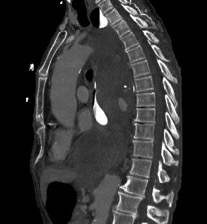
\includegraphics[width=.9\textwidth]{images/ct_compression_oesophagienne.jpg}
        \caption{flèche bleu: lumière oesophagienne comprimé; H: hématome; o: œsophage}
        \label{subfig:ct_1}
    \end{subfigure}%
%
    \begin{subfigure}[b]{.5\textwidth}
        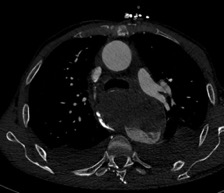
\includegraphics[width=.9\textwidth]{images/ct_lumieres_oesophagienne_et_aortique.jpg}
        \caption{flèche bleu: lumière oesophagienne; H: hématome; Ao: lumière aortique}
        \label{subfig:ct_2}
    \end{subfigure}
    
    \caption{Compression oesophagienne par hématome vu en CT de thorax}
    \label{fig:ct_thorax}
\end{figure}

Une échographie cardiaque réalisée a exclu une insuffisance ventriculaire tout en montrant des variations des pressions de remplissage cardiaque dues à la compression par l'hématome.

Pendant son séjour à l’USI, le patient a eu des épisodes de broncho-aspiration nécessitant la mise en place de sonde naso-gastrique. Une gastrostomie a été posée pour la nutrition. Par la suite, développement des épisodes de FA traités par du Cordarone, apparition de l’hématémèse, persistance de broncho-aspiration et développement de l’insuffisance respiratoire aigüe. La bactériologie de sécrétions trachéales a mis en évidence E. Coli et P. Mirabilis traités par Zinacef et Tazocin. Au J26, suite à un nouvel épisode de broncho aspiration, une œsophago-gastro-duodénoscopie réalisée a montré une œsophagite érosive, un pont muqueux dans l'œsophage thoracique et une impaction alimentaire locale. Répétée 3 jours plus tard, l’OGD (Fig3) a démontré plusieurs fistules permettant même de visualiser le poumon droit en suivant le trajet fistuleux. Le Ct thoracique du J38 a confirmé la fistule œsophagienne par la fuite de gastrographine dans l’hématome aortique (Fig4).

Dans une tentative de placement d’une prothèse au J56, découverte d’une lésion œsophagienne de 10 cm de long impossible à couvrir par un stent. Un geste chirurgical a été proposé et a consisté en une exclusion de l'œsophage thoracique. Ainsi le 12 avril 2019, a été réalisé une exclusion œsophagienne (Fig.5) avec œsophagostomie cervicale gauche, une jéjunostomie d’alimentation, une pyloroplastie ainsi qu’une séparation cardio-œsophagienne avec une bonne évolution postopératoire. Un abcès sur le site de l’ancienne gastrostomie par du P. Aeruginosa a été traité avec du Méropenem 1g  3 fois par jour associé à du Fluconazole 400mg une fois par jour et Linézolide 600mg 2 fois par jour. Le patient était confortable et s’était bien adapté à la nutrition par jéjunostomie tout en appréciant de boire à nouveau per os.


\begin{figure}[!h]
    \centering
    \begin{minipage}[b]{.5\textwidth}
        \centering
        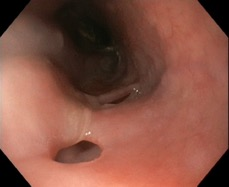
\includegraphics[width=.95\textwidth]{images/endoscopie.jpg}
        \caption{visualisation de 2 fistules sur OGD J26.}
        \label{fig:endoscopie}
    \end{minipage}%
%
    \begin{minipage}[b]{.5\textwidth}
        \centering
        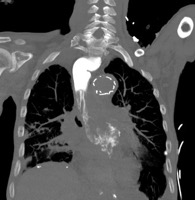
\includegraphics[width=.95\textwidth]{images/ct_fuite_de_grastrographine.jpg}
        \caption{fuite de gastrographine en moulant.}
        \label{fig:fuite_grastrographine}
    \end{minipage}
\end{figure}

\begin{figure}[ht]
    \centering
    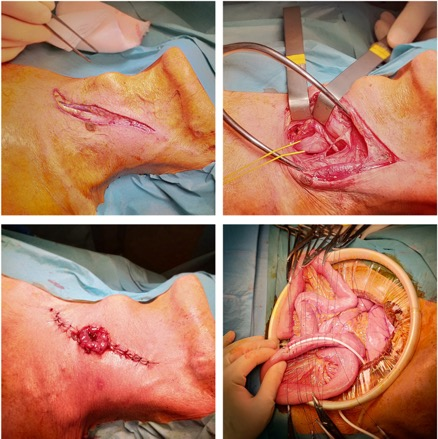
\includegraphics[width=\textwidth]{images/chirurgie.jpg}
    \caption{A : incision sur le bord antérieur du muscle sternocleido-mastoïdien ; B :tête de flèche indique un lacs jaune utilisé pour isoler l’œsophage cervical ; C : fistule oesophagienne confectioné en positio cervico-latérale gauche ; D : Confection de jejunostomie.}
    \label{fig:chirurgie}
\end{figure}

Au 72ème jour d’hospitalisation, le patient a présenté une clinique de détresse respiratoire aiguë et est décédé dans la nuit. Aucune autopsie n'a été réalisée.

\end{document}